
\section{Slum Formation}
The idea of a slum has been around since the conception of urbanized areas. There are various definitions that often differ from city to city but are generally along the lines of a dense cluster of informal housing units where living conditions are bad: these areas are usually associated with poverty, a lack of hygienic conditions, and a lack of land ownership upon which families take shelter. Although the concept of a slum itself has yet to have a widely adopted definition, in 2002 the UN-Habitat agreed upon an internationally recognized definition for a slum household as 
\begin{quoting}
one in which the inhabitants have one or more of the following household deprivations: (1) Lack of access to improved water sources, (2) Lack of access to improved sanitation facilities, (3) Lack of sufficient living area, (4) Lack of household durability, and (5) Lack of security of tenure\textsuperscript{\cite{UNslumdef}}.
\end{quoting}

How slums tend to emerge is an issue that is currently being studied. At a higher macro level, Henderson (2002)\textsuperscript{\cite{Henderson}} indicates that often times a mismatch in the rate of urbanization and investment capital available to a city leads to overcrowding, excessive traffic, and significant health costs due to air and water pollution: characteristics of a city that not only incentives slum growth but also make slums more dangerous for the people living in them. This is a key issue for developing countries right now, such as countries in sub-Saharan Africa and South Asia, which are urbanizing at a rate much faster than developed countries.

India, for example, has seen rapid urbanization in recent years and 29.4\% of its population lives in slums, while the percentage of slum dwellers reached 42\% in Mumbai, the largest city and financial capital of the country\textsuperscript{~\cite{MTSU}}. Further, in Rio de Janeiro, although the city's total population grew only 3.4\% over the last decade, the favela population has grown by 27.7\% \textsuperscript{\cite{LuiZhang}}. The case of China is a clear example of the opposite side of the story where there are cities whose infrastructure expenditure has outpaced the rate of urbanization, and as a result, experience a relative lack of slums compared to the megacities in China's developing country counterparts. Lui and Zhang\textsuperscript{\cite{LuiZhang}} explain, however, that China's dual-track urbanization of first government-driven spatial expansion of cities and related infrastructure and second farmer-driven urbanization through the construction of housing after their cropland is lost to city expansion keeps the supply of housing high enough to accommodate migrant workers who may have otherwise been living in slums.

\begin{figure}
    \centering
    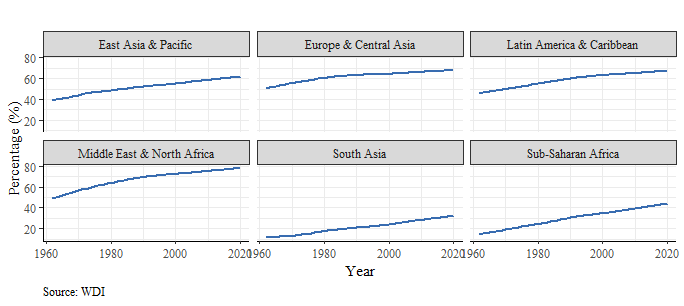
\includegraphics[scale = 0.8]{Graphics/urbanpopPercent.png}
    \caption{Average percent of people living in urban areas has been growing in regions around the world.}
    \label{fig:Urbanpopgrowth}
\end{figure}

Urbanization seems to trend according to the stage of development that nations are currently experiencing. Despite this, the fact remains that countries at every income class on average experience urban population growth rather than a decline (Figure 1). Slum populations on average as a proportion of urban populations, however, seem to be paradoxically decreasing (Figure 2). 

Although this is an aggregate trend and may not be the case in every country, it still raises questions about the factors that influence slum growth. Additionally, even though infrastructure spending seems to have on average experienced an upwards trend across regions relative to past decades (Figure 3), this trend doesn't seem to correlate well with the relative magnitudes of slum decline and some regions that don't experience any increase in infrastructure spending to match growing urban areas also witness a decline in slum proportions amongst urban populations.

\begin{figure}
    \centering
    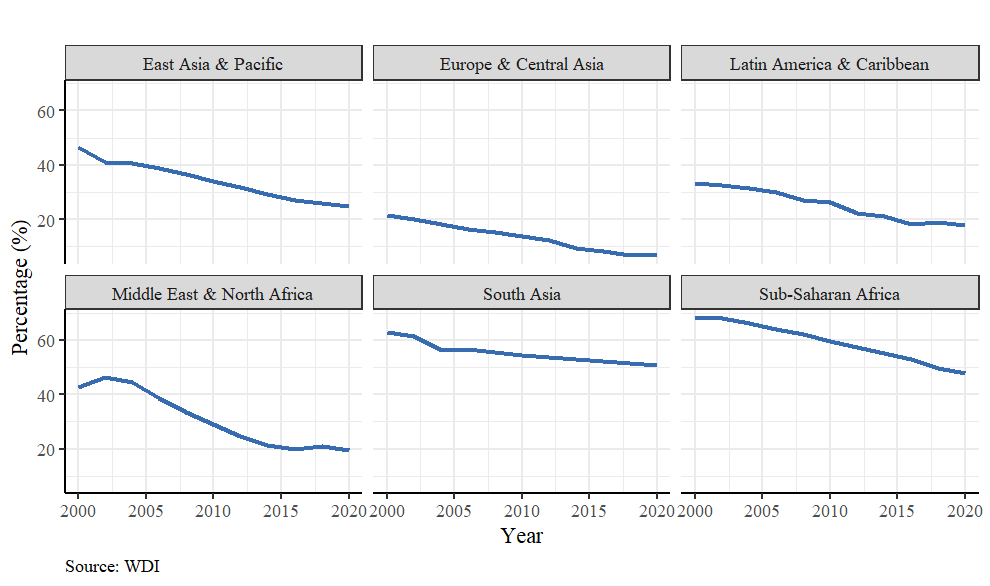
\includegraphics[scale = 0.8]{Graphics/Average Percent of urban households living in slums.png}
    \caption{Average percent of urban households living in slums has been on the decline in every global region.}
    \label{fig:SlumsTrend}
\end{figure}

\begin{figure}
    \centering
    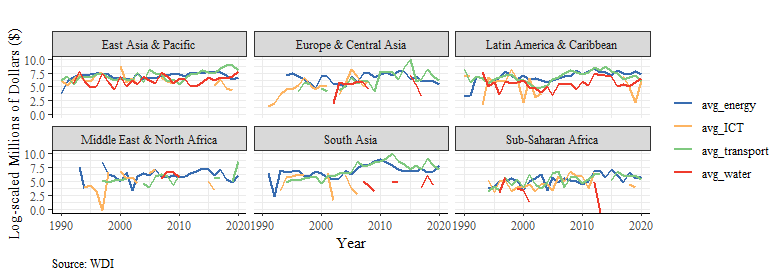
\includegraphics[height = 6cm]{Graphics/Average country-wide infrastructure spending per region.png}
    \caption{Average country-wide infrastructure spending per region}
    \label{fig:Infraspending}
\end{figure}

\begin{table}[ht]
\centering
\caption{Estimated total stocks of migration from, to, and within Africa\textsuperscript{{\cite{WBGBMD}}}}
\begin{tabular}{rlll}
  \hline \hline 
 & Africa to the rest of the world & Rest of the world to Africa & Within Africa\\ 
  \hline
1960 & 1 830 776 & 2 811 930 & 6 176 385 \\ 
1980 & 5 418 096 & 1 872 502 & 7 966 359  \\ 
2000 & 8 734 478 & 1 532 746 & 10 500 000  \\ 
   \hline
\end{tabular}
\end{table}

Despite their prevalence across the world, slums all have varying characteristics from region to region. This project, however, is focused on Sub-Saharan Africa since that is where most of the training data has been collected and is the region with the second-highest average proportion of urban populations living in slums. Urban movement in Africa is often miss-classified as a mass exodus from Africa to Western Nations, in fact, Africa has the lowest intercontinental out-migration rates of all world regions\textsuperscript{\cite{Teye}}. Although intercontinental migration, especially to Europe, has been on the rise in Africa itself, this has been primarily focused in North Africa and still pales relative to intracontinental migration within Africa itself which has also been increasing (Table 1). 


These migration patterns have a significant effect on the urban landscape in Africa. As is generally the case around the world, migration mobility in Africa has been seen to be linked to the wealth of a given country and its habitants. The wealthier an individual, the more facility they have to relocate, and relocate to further distances as well. This is why a significant proportion of urban movement lies within rural relocation to urban areas in search of greater opportunity. Teye explains that 
\begin{quoting}although a significant proportion of the rapid increase in urban population is caused by the high rate of natural increase in towns and re-classification of settlements into urban areas, migration accounts for a significant proportion urbanization in Africa. In some countries, rural-urban migration accounts for about 60\% of urban growth because rural-urban inequalities of development force people to move from rural areas to urban areas in search of jobs \textsuperscript{\cite{Teye}}.\end{quoting} 

The packing of poor groups of people into already overburdened urban areas due to the migratory movement of rural peoples into urban areas is what this paper studies. A significant amount of this paper will focus on Kenya, so it is important to take a cursory look at the migratory characteristics of Kenya as well. Figure 4 shows how urban population growth in Kenya has stayed fairly consistently positive over the past 30 years but slum proportions have been on the decline since 2000 (Figure 5). Infrastructure spending data in Kenya is sparse and is not enough to conclude some sort of trend.

\begin{figure}
    \centering
    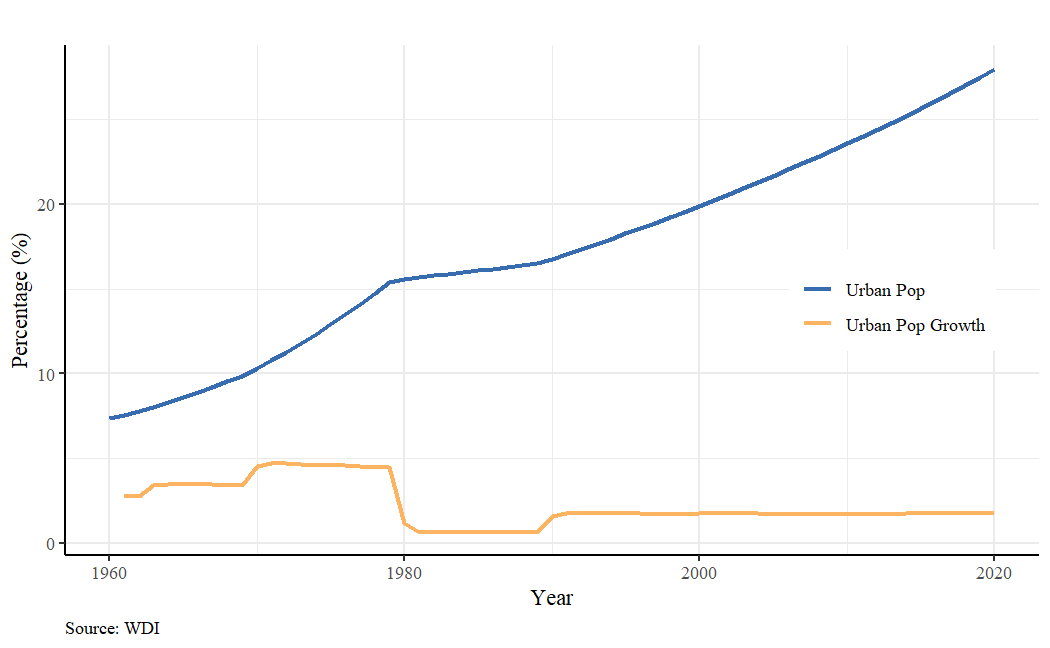
\includegraphics[scale = 0.65]{Graphics/Kenya Urban Population Percentage.png}    
    \caption{Urban population growth as a percentage of the total population of Kenya has stayed fairly consistent over the past 20 years.}
    \label{fig:KenyaUrban}
\end{figure}


\begin{figure}
    \centering
    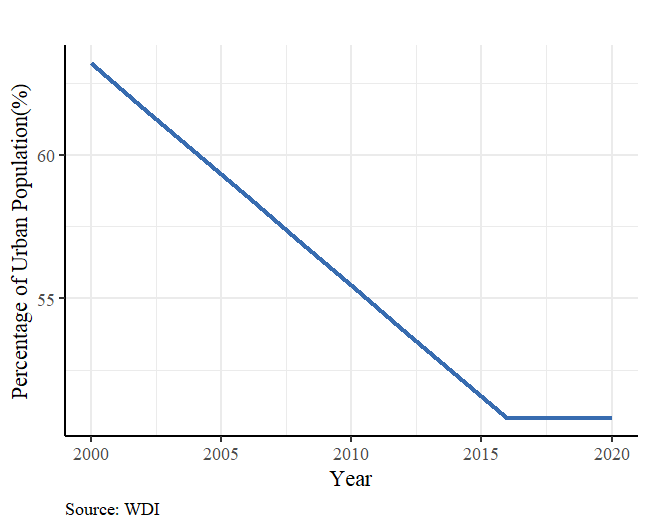
\includegraphics[scale = 0.8]{Graphics/Kenyan Urban Slums.png}
    \caption{Despite urban population growth, the slum proportion of urban populations has been on the decline}
    \label{fig:kenyanslums}
\end{figure}



